\documentclass{article}

\usepackage[latin1]{inputenc}
\usepackage[brazil]{babel}

\usepackage{Sweave}
\begin{document}
\Sconcordance{concordance:aula3.tex:aula3.rnw:%
1 5 1 1 0 9 1 1 8 4 1 2 3 10 1 1 40 1 3 12 1 1 58 1 3 3 1}


\section{Aula 3 - 17/03/2017}

%#########################################

\subsection{Primeira Parte}
Introducao ao ambiente RStudio.


O grafico da funcao seno e apresentado na Figura \ref{Fig1}
\setkeys{Gin}{width=0.6\textwidth}
\begin{figure}[h]
\centering
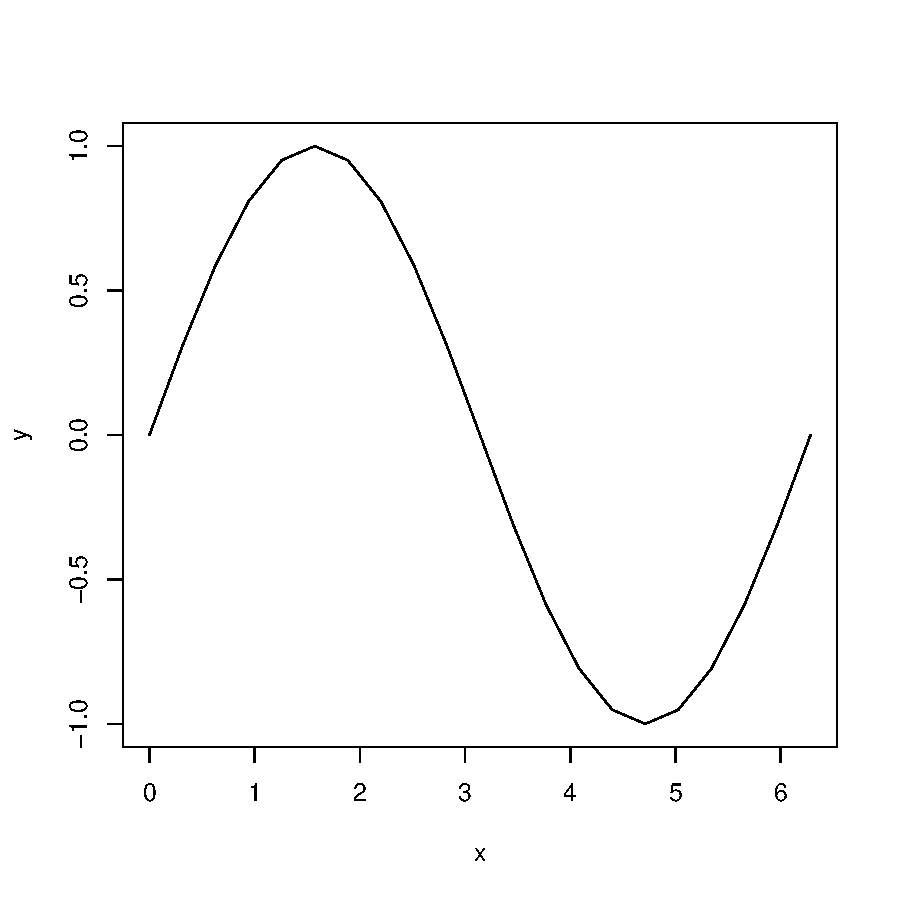
\includegraphics{aula3-002}
\caption{Grafico da funcao seno}
\label{Fig1}
\end{figure}

%#########################################

\subsection{Classificador Univariado}

\setkeys{Gin}{width=0.6\textwidth}
\begin{figure}[h]
\centering
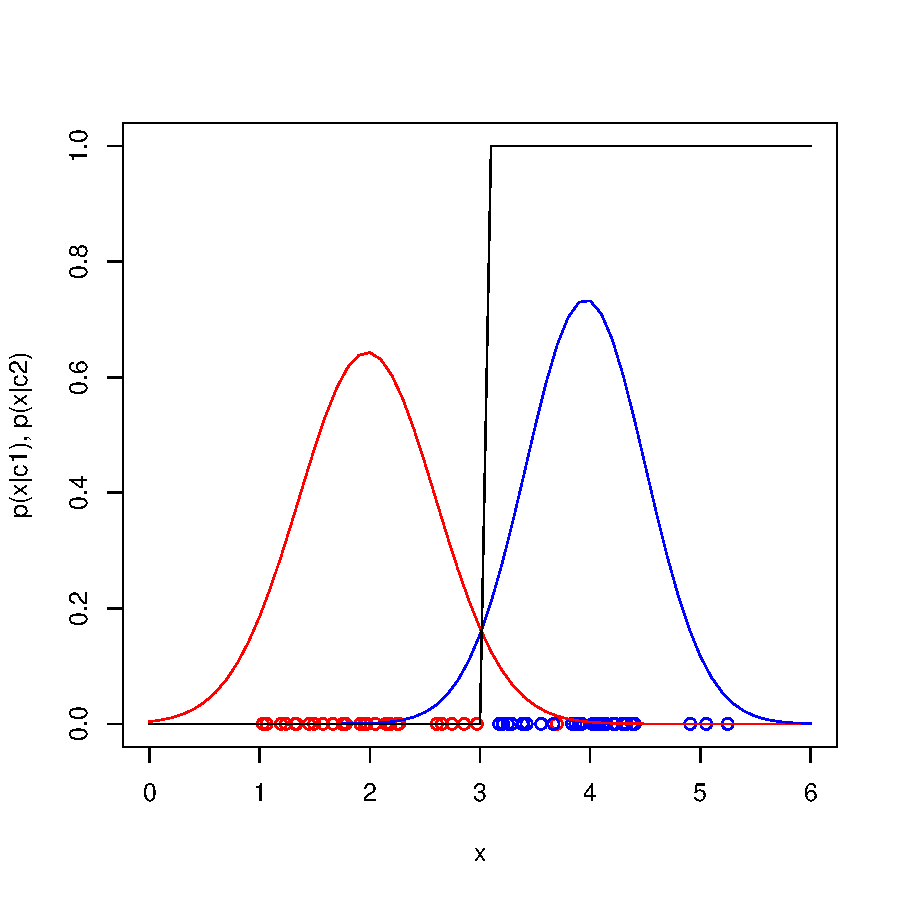
\includegraphics{aula3-003}

\caption{Classificador univariado}
\label{Fig2}
\end{figure}

%#########################################

\subsection{Problema: Densidade conjunta}

Problema: 1 das classes nao e unimodal. Gerar conjunto de dados:
Gerador:
-> medias: 2, 3, 4
Supor que as amostras são conhecidas. Densidade conjunta e a mistura das densidades.

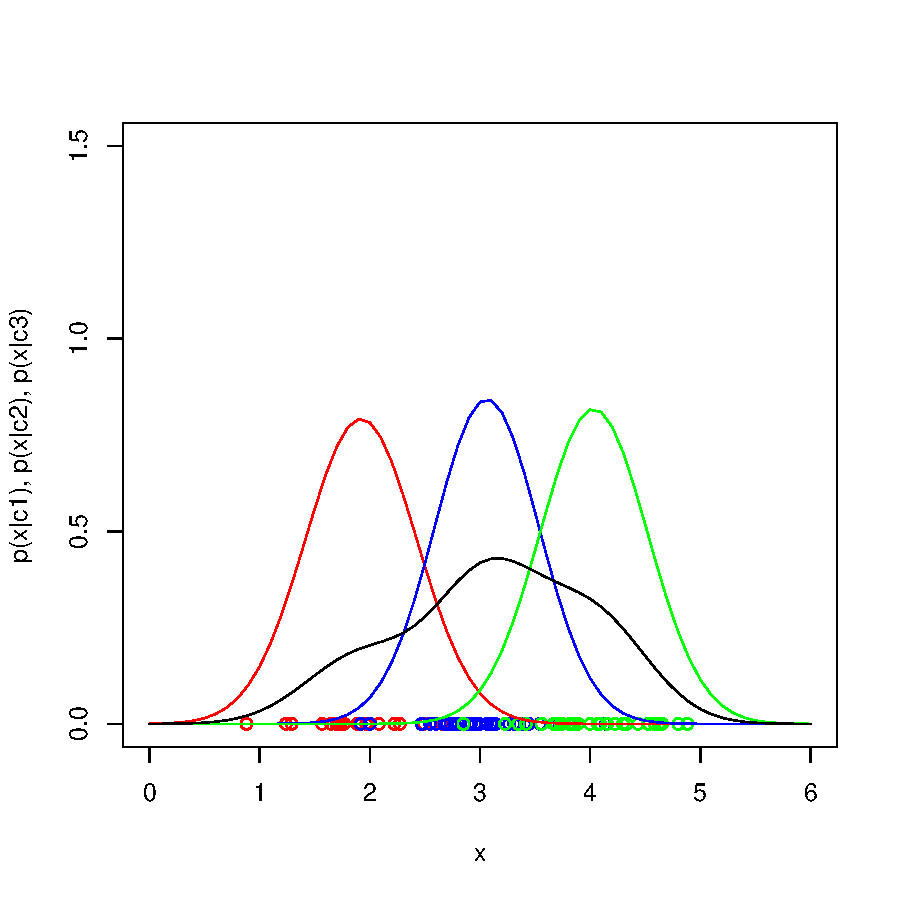
\includegraphics{aula3-004}

%#########################################

\subsection{Distribui��o bimodal}


\begin{Schunk}
\begin{Sinput}
> rm(list=ls())
> fnormal1var <- function(x,m,r)
+ {
+   y <- (1/(sqrt(2*pi*r*r)))*exp(-0.5*((x-m)/(r))^2)
+   return(y)
+ }
> ###########################
> 
> c1 <- matrix(rnorm(100, mean = 2, sd = 0.6), nrow=2)
> c2 <- matrix(rnorm(100, mean = 4, sd = 0.6), nrow=2)
> plot(c1[,1], c1[,2], matrix(0, nrow=100, ncol=1), col='red', type='p', xlim=c(0,6), ylim=c(0,1.5), xlab='',ylab='')